\chapter{Results and Discussion} \label{chap_results}

\section{Results}

The architecture of Imagezor was fully implemented and tested in simulation, but unfortunately it was not tested on actual hardware. But by making some assumtions we can estimate a theoretical performance. From Section \ref{architecture} we know that since the convoluter is the one that feeds data to the other components, and that they use one cycle to process the data, that it is the deciding factor for the performance. The convoluter uses $ k \times k $ cycles to load the kernel weights, and $ n \times n $ cycles to compute one convolution.  Using this we can define the metric \textit{conv\_net\_op/s}, which is how many subsampled/pooled feature map the application can compute per second, i.e. the basic operation of Imagezor. Since we used a Spartan 6, which only have resources enough for a single instance of Imagezor, this theorectial performance will only consider one instance of the Imagezor architecture.  

We can thus define the performance of Imagezor as:

\begin{equation} \label{eq_theoretical_performance}
\frac{f}{I\times(n \times n) + (k \times k) + 5} ~conv\_net\_op/s
\end{equation}

Where \textit{f} is the expected clock frequency of the architecture, and \textit{I} is the number of images that is required to compute a subsampled/pooled feature map. 

Using Equation \ref{eq_theoretical_performance} the Imagezor architecture was  compared  to a Intel Core i5-450. The CPU executed a C program which performed all the operations of the convolution and subsample/pooling layer. The program was run and timed 1000 times for each configuration of the input and kernel size, and the average time was used for comparison. We could then calculate the C program's conv\_net\_op/s by simply by dividing one second by the average time used.  In order to compare the scalability both different images sizes and kernel sizes was tested. The results from comparing the theoretical performance for Imagezor against the C program is shown in Figure \ref{fig_cpu_cmp_results}.
\begin{figure}
  \centering
      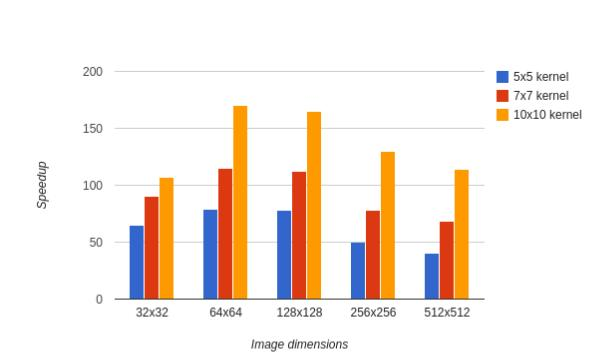
\includegraphics[width=0.6\textwidth]{Figures/Results/Speedup_chart}
  \caption{The theoretical speedup our module had compared to a Intel Core i5.}
  \label{fig_cpu_cmp_results}
\end{figure}

As can be seen by the figure, Imagezor can be up to 170x faster than the CPU, i.e. was able to perform 170x more conv\_net\_ops per second. This makes a good case for accelerating the network operations in hardware. We can also see that even with limited hardware resources of the Spartan 6, only able to support a $ 5 \times 5 $ kernel, the speedup is still significant, up to 75x speedup.

In addition the Intel Core uses 85 W, while the Spartan 6 uses about 1.5 W. Using this we can calculate conv\_net\_op/joule by dividing conv\_net\_op/s by the power usage. 

\section{Discussion}

The results from the previous section makes a strong case for hardware accelerating the convolution and subsample/pooling layer in a Convolution Layer. We see that even with hardware that only supports a $ 5 \times 5 $ kernel and does not exploit intra- and inter-parallelism found in the network, the speedup is significant, and the energy effiency is up to 1000x better. 

We see that the speedup scales with the size of the kernel. This makes sense since Imagezor primarly exploits the parallelism in the convolution operation, by computing effectively $ k \times k $ pixels at once. In addition the subsample/max-pooling does not take any additional time since it is able to process the pixels as fast as the convoluter module is able to deliver them.   
